\documentclass{./../div_teaching_slides}
\usepackage{setspace}

\begin{document}
\title{ECON 340 \\ Economic Research Methods}
\author{Div Bhagia \\\vspace{1.75em}
Lecture 4 \\\vspace{0.25em} \small Covariance and Correlation}
\date{}

\begin{frame}[noframenumbering, plain]
\maketitle
\end{frame}

%%%%%%%%%%%% 
\begin{frame}{Where would you want to live?}
\centering \vspace{-0.5em}
\begin{tabular}{cc}
Mushroom Kingdom  & Bowser's Kingdom \\
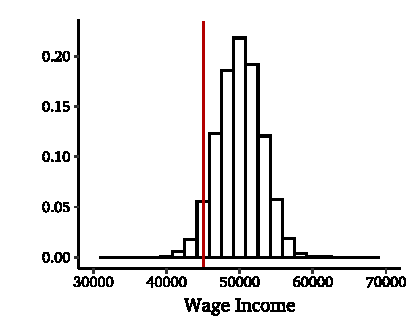
\includegraphics{./../../Output/income_mk_z.pdf} &
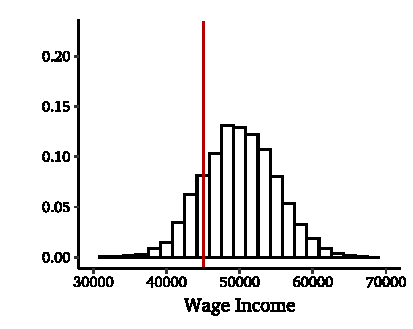
\includegraphics{./../../Output/income_bk_z.pdf} \\ 
Mean = Median= \$50,000 & Mean = Median= \$50,000 \\
SD= \$3,000 & SD= \$5,000 \\
\end{tabular}
\end{frame}

%%%%%%%%%%%% 
\begin{frame}{Z-Score}
We can calculate the Z-Score to capture how many standard deviations ($\sigma$) away from the mean ($\mu$) a specific observation is. \\
$$ Z = \frac{X - \mu}{\sigma} \quad \rightarrow \quad X = \mu + Z.\sigma $$ \\~\\
Example: $\sigma_{MK} = 3000$, $\sigma_{BK} = 5000$ \\
 $$Z_{MK} = \frac{45000 - 50000}{3000} = -1.66 \quad \quad Z_{BK} = \frac{45000 - 50000}{5000} = -1$$ \\~\\
\end{frame}

%%%%%%%%%%%% 
\begin{frame}{Describing Data}
\textit{How do we summarize the information contained in a variable?} \\
\begin{witemize}
\item Empirical distribution, histogram, percentiles 
\item Measures of central tendency: mean, median, mode
\item Measures of variance: range, variance, standard deviation \\~\\
\end{witemize}
\textit{How do we summarize the relationship between two variables?} \\
\end{frame}


%%%%%%%%%%%% 
\begin{frame}{}
\centering
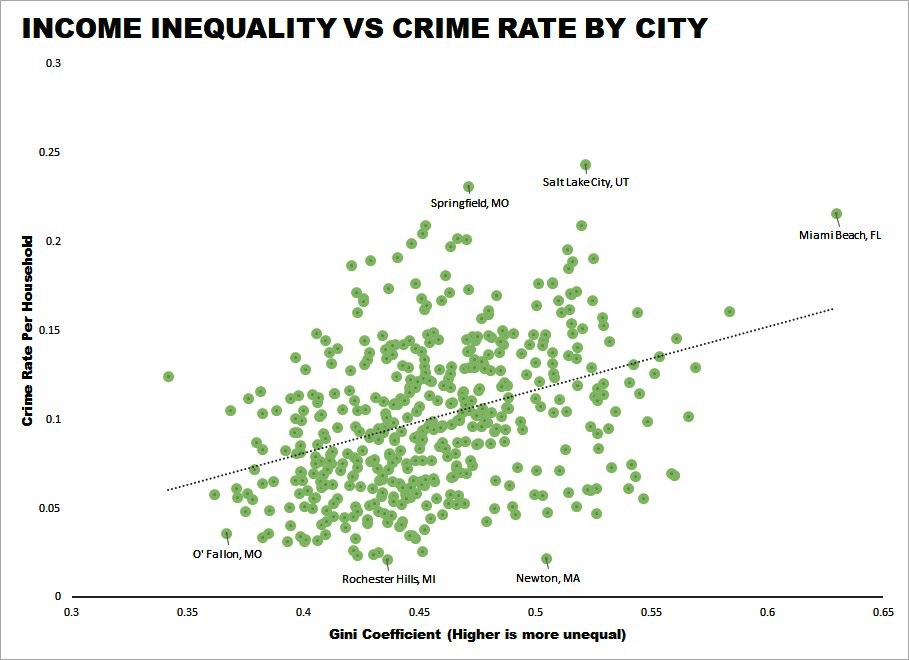
\includegraphics[scale=0.625]{crime}
\end{frame}

%%%%%%%%%%%% 
\begin{frame}{Describing Relationships}
\begin{witemize}
  \item Scatterplot: a graph where each point represents an observation of two variables
  \item Can see the relationship between two variables
  \item Positive relationship if when $X$ is high $Y$ is high (and when $X$ is low $Y$ is low)
  \item Negative relationship if when $X$ is high $Y$ is low (and when $X$ is low $Y$ is high)
  \item \textit{How to construct a statistic to capture this?}
\end{witemize}
\end{frame}

%%%%%%%%%%%% 
\begin{frame}{Covariance}
Covariance indicates whether there is a positive or negative relationship between two variables. 
$$ \sigma_{XY} = \frac{1}{N}\sum_{i=1}^N (X_i-\mu_X)(Y_i-\mu_Y) \quad (Population) $$
$$ S_{XY} = \frac{1}{n-1}\sum_{i=1}^n (X_i-\bar{X})(Y_i-\bar{Y}) \quad (Sample) $$
\end{frame}

%%%%%%%%%%%%%%%%%%%%
\begin{frame}{Example}
\vspace{-0.25em}
$X_i$: sleep in hours, $Y_i$: exercise in hours \\~\\
\begin{tabularx}{1\textwidth}{P{1.5cm}P{1.5cm}P{1.5cm}Y}
\hline \addlinespace[0.5em]
Week & $X_i$ & $Y_i$ & $(X_i-\mu_X)(Y_i-\mu_Y)$   \\ \addlinespace[0.5em] \hline \addlinespace[0.5em]
1 & 6 & 0.5 &    \\ \hline \addlinespace[0.5em]
2 & 9 & 0.3 &    \\ \hline \addlinespace[0.5em]
3 & 9 & 1 &    \\ \hline \addlinespace[0.5em]
 Total & & & \\
 \hline 
\end{tabularx} 
$$ \sigma_{XY} = \frac{1}{N}\sum_{i=1}^N (X_i-\mu_X)(Y_i-\mu_Y) = \hspace{5cm} $$
\end{frame}


%%%%%%%%%%%%%%%%%%%%
\begin{frame}{Why does the formula work?}
\centering
\begin{tikzpicture}
% Draw x and y axis
\draw[<->, line width = 0.6pt] (-1,0) -- (8,0) node[below] {\(X\)};
\draw[<->, line width = 0.6pt] (0,-1) -- (0,6) node[left] {\(Y\)};

% Draw Y-bar
\draw[dotted, line width = 1.25pt] (-1,3) -- (8,3);

% Draw y-bar
\draw[dotted, line width = 1.25pt] (4,-1) -- (4,6);

% Label the quadrants
%\node at (6,5.25) {\small I};
%\node at (2,5.25) {\small II};
%\node at (2,2.25) {\small III};
%\node at (6,2.25) {\small IV};

% Selected nodes
\draw (0,0) -- (0,0) node[below left] {\(0\)};
\draw (4,0) -- (4,0) node[below right] {\(\bar{X}\)};
\draw (0,3) -- (0,3) node[below left] {\(\bar{Y}\)};
\end{tikzpicture}
\end{frame}

%%%%%%%%%%%% 
\begin{frame}{Correlation}
Correlation also indicates the \textit{strength} of the relationship in addition to the \textit{direction}.
$$ \rho_{XY} = \frac{ \sigma_{XY}}{\sigma_X \sigma_Y}  \quad (Population) \quad \quad r_{XY} = \frac{ S_{XY}}{S_X S_Y} \quad (Sample) $$ \\~\\

Bounded between -1 and 1. 
\begin{itemize}
  \item $\rho = 0$, no linear relationship
  \item $\rho = 1$, perfect positive linear relationship
  \item $\rho = -1$, perfect negative  linear relationship
\end{itemize}

\end{frame}

%%%%%%%%%%%%%%%%%%%%
\begin{frame}{Correlation}
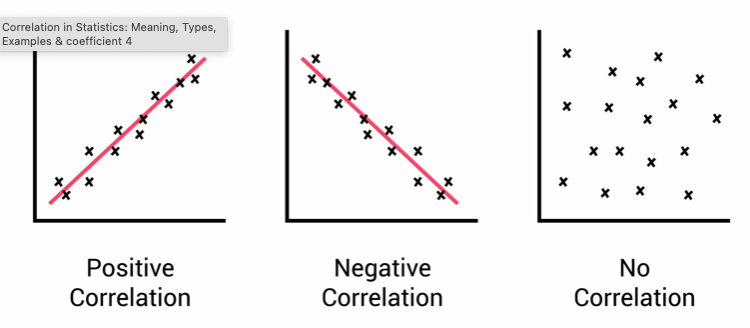
\includegraphics[scale=0.525]{corr}
\end{frame}


%%%%%%%%%%%%%%%%%%%%
\begin{frame}{Example}
\vspace{-0.25em}
$X_i$: sleep in hours, $Z_i$: exercise in minutes \\~\\
\begin{tabularx}{1\textwidth}{P{1.5cm}P{1.5cm}P{1.5cm}Y}
\hline \addlinespace[0.5em]
Week & $X_i$ & $Z_i$ & $(X_i-\mu_X)(Z_i-\mu_Z)$   \\ \addlinespace[0.5em] \hline \addlinespace[0.5em]
1 & 6 & 30 &    \\ \hline \addlinespace[0.5em]
2 & 9 & 18 &    \\ \hline \addlinespace[0.5em]
3 & 9 & 60 &    \\ \hline \addlinespace[0.5em]
 Total & & & \\
 \hline 
\end{tabularx} 
$$ \sigma_{XZ} = \frac{1}{N}\sum_{i=1}^N (X_i-\mu_X)(Z_i-\mu_Z) = \hspace{5cm} $$
\end{frame}


%%%%%%%%%%%% 
\begin{frame}{Finally... Correlation is not causation}
A positive correlation between inequality and crime doesn't suggest that inequality $\rightarrow$ crime. This is for two reasons: \\~\\
\begin{witemize}
  \item \textit{Reverse causality}: crime $\rightarrow$ inequality (unlikely here but a concern in many situations)
  \item \textit{Other confounding factors}: larger, more congested cities tend to be more unequal and also have higher crime rates
\end{witemize}
\end{frame}


%%%%%%%%%%%%%%%%%%%%
\begin{frame}{Things to do next}
\begin{witemize}
\item Install R and R Studio on your computers if you haven't already (instructions on the course website)
\item Please read Chapter 1 from Stock \& Watson (uploaded on Canvas). We will discuss it on Tuesday. 
\item Finalize the research project team by end of the day
\item Coming up: Problem Set 1 (Due on Tues)
\end{witemize}
\end{frame}

\end{document}